\chapter{Problem Formulation}\label{ch:problem}
\section{Graphs, identities, and partitions}
Let $U$ be a fixed finite public universe of stable identities. A legal training graph is $G=(V,E)$, where $V\subseteq U$ and $E\subseteq V\times V$. The fixed mechanism domain excludes self-loops and duplicate edges. Isolated surviving nodes remain valid. For directed inputs, $(u,v)$ is an outgoing edge from $u$ to $v$; undirected inputs require the corresponding frozen representation rather than an implicit change in direction.

The prepared experimental data have disjoint training and test identities. A decoder maps file-local IDs to stable identities. The theoretical adjacency below acts on decoded graphs; arbitrarily deleting a line from an edge file need not create the required adjacent input because file membership, isolated nodes, and decoding can change. The existing mappings and graph structures are preserved throughout the experiments.

The 50:50 preparation rule is the original split procedure, not a statement that the final active-node totals or edge counts are identical between partitions. Filtering and removal of cross-partition edges can produce unequal counts. In particular, the fixed public Email universe contains 1005 identities, while the saved prepared training and test graphs contain 462 and 458 active nodes. The public identity universe must not be reconstructed from the current private vertex set.

\section{Seed selection and Coverage}
For a graph $G=(V,E)$ and a seed budget $k$, the generic influence-maximization objective is
\begin{equation}
 \max_{\substack{S\subseteq V\\ |S|\leq k}}
 \mathbb{E}\!\left[|\mathcal{A}(S;G)|\right],
 \label{eq:im-objective}
\end{equation}
where $\mathcal{A}(S;G)$ is the set of active vertices, including the seeds, at the end of the specified diffusion process. The expectation is over the randomness of that process \cite{kempe2003}.

For a test graph $G^{\mathrm{test}}$, a scoring model $f_\theta$ gives a real-valued score to each candidate. The selected set $S_\theta$ contains the 50 highest pre-sigmoid scores, using the original stable local-ID rule for ties. Let $N^+(v)$ denote outgoing neighbors in the test graph. The implemented evaluation runs one step of the independent cascade process along outgoing edges with transmission probability one, so the spread is deterministic:
\begin{equation}
 \operatorname{Spread}(S;G^{\mathrm{test}})
 =\left|S\cup\bigcup_{v\in S}N^+(v)\right|.\label{eq:spread}
\end{equation}

For graph $d$, let $c_d$ be the frozen CELF reference spread. The reported outcome is
\begin{equation}
 Y_{dmi}=100\frac{\operatorname{Spread}_{dmi}}{c_d},\label{eq:coverage}
\end{equation}
where $m$ denotes configuration and $i$ a complete repeat. Coverage is measured as a percentage of the reference, while a difference in Coverage is measured in percentage points. Coverage is not the percentage of all test nodes. Since the reference need not be a global optimum, $Y$ is not assumed to be bounded by 100; the public conservative bound is $0\leq Y\leq100|U_d|/c_d$.

\subsection{Effect of exchanging a ranked seed}
The relationship between ranking and Coverage can be made explicit for the deterministic evaluation in Equation~\eqref{eq:spread}. Write $B(v)=\{v\}\cup N^+(v)$ for the vertices reached by a seed $v$, and let $R=\bigcup_{s\in S\setminus\{u\}} B(s)$ be the vertices reached by the seeds shared between two selections. Replacing selected node $u$ with an unselected node $v$ gives $S'=(S\setminus\{u\})\cup\{v\}$ and changes Coverage by
\begin{equation}
 \frac{100}{c_d}
 \bigl(|B(v)\setminus R|-|B(u)\setminus R|\bigr).
 \label{eq:coverage-exchange}
\end{equation}
The common coverage $|R|$ cancels. The sign and magnitude depend on the reach of the exchanged seeds beyond $R$. Two candidates with very similar scores may have different contributions to this union, and even completely disjoint seed sets can have the same spread. Coverage and overlap of selected identities therefore answer different questions about a ranking.

A deterministic score margin can certify whether a bounded score change preserves the selected set on a fixed graph. Let $z_{(k)}$ and $z_{(k+1)}$ be the ordered scores at the selection boundary. Suppose every score changes by at most $\eta$ in absolute value. If $z_{(k)}-z_{(k+1)}>2\eta$, every originally selected score still exceeds every originally unselected one. The selected set and its spread are then unchanged. At equality a boundary tie can occur. When the gap is smaller, a crossing is possible, and Equation~\eqref{eq:coverage-exchange} describes the utility effect if exactly one pair exchanges membership. The margin statement is conditional on the score perturbation bound. It supplies neither a bound on scores from Gaussian training nor an empirical explanation of any particular run.

\section{Node adjacency and personalized protection}
\begin{definition}[Fixed-domain node add/remove adjacency]
For $v\in V$, $G-v$ removes $v$ and every incident edge, preserves all surviving stable identities and their edges, and retains surviving isolated nodes. The graphs $G$ and $G-v$ are adjacent with respect to identity $v$. The public $U$, Registry, and all truly public auxiliary information remain unchanged.
\end{definition}

This is a node-membership and incident-structure relation, not edge adjacency. It does not protect uncertainty about whether an identity is in the public universe; that universe is conditioned upon. Within the actual training domain, test identities are excluded from training inputs. A target label assigned to a held-out identity does not thereby establish privacy of its test graph.

Let $\mathcal{R}$ be the fixed public Registry, containing the target pair $(\epsilon^{\mathrm{tar}}_v,\delta^{\mathrm{tar}}_v)$ for every $v\in U$. In this study $\epsilon^{\mathrm{tar}}_v\in\{1,2,4\}$ and $\delta^{\mathrm{tar}}_v=10^{-5}$. Policy labels themselves are public assumptions, not secretly learned preferences protected by the model theorem.

\begin{definition}[Conditional personalized Node-DP]
A mechanism $M$, conditional on fixed public auxiliary information, satisfies per-identity bounds $(\epsilon_v,\delta_v)$ if, for every legal node-adjacent pair and every measurable output event $F$,
\begin{align}
 \Pr[M(G)\in F]&\leq e^{\epsilon_v}\Pr[M(G-v)\in F]+\delta_v,\\
 \Pr[M(G-v)\in F]&\leq e^{\epsilon_v}\Pr[M(G)\in F]+\delta_v.
\end{align}
Meeting the target policy requires $\epsilon_v\leq\epsilon^{\mathrm{tar}}_v$ and $\delta_v\leq\delta^{\mathrm{tar}}_v$.
\end{definition}

The numbers supplied by the accountant are sufficient upper bounds. They are not a measurement of exact realized privacy loss and are not asserted to be the smallest possible guarantees. Sharing the same policy caps does not mean two mechanisms have equal actual privacy losses.

\subsection{Node removal in an objective and in a learned decision}
Node adjacency changes several graph objects at once. For example, take the seed $s$, an intermediate vertex $v$, and vertices $x_1,\ldots,x_m$, with edges $(s,v)$ and $(v,x_i)$ for every $i$. All edges transmit with probability one. Under the two-step cascade, the fixed seed $\{s\}$ covers all $m+2$ vertices. Removing $v$ reduces the spread to one: $s$ and all surviving $x_i$ remain present, yet their connecting paths from $s$ disappear. The same removal under the one-step cascade reduces the spread from two to one.

\begin{figure}[htbp]
\centering
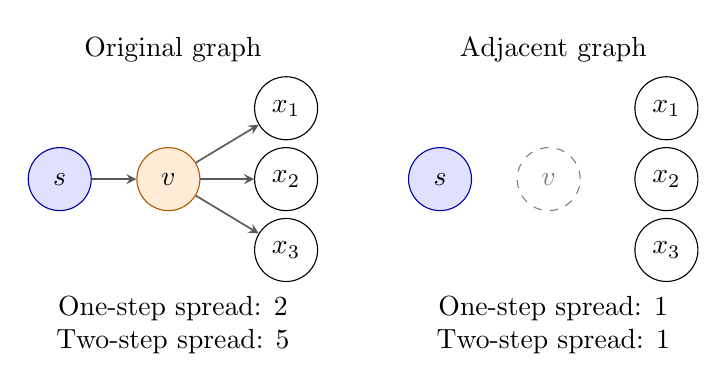
\begin{tikzpicture}[
 x=1.15cm,y=1cm,
 vertex/.style={circle,draw,minimum size=8mm,inner sep=0pt},
 seed/.style={vertex,draw=blue!65!black,fill=blue!12},
 relay/.style={vertex,draw=orange!70!black,fill=orange!16},
 arc/.style={->,>=stealth,semithick,draw=black!65}]
 \node[seed] (s) at (0,0) {$s$};
 \node[relay] (v) at (1.2,0) {$v$};
 \node[vertex] (a) at (2.5,0.9) {$x_1$};
 \node[vertex] (b) at (2.5,0) {$x_2$};
 \node[vertex] (c) at (2.5,-0.9) {$x_3$};
 \draw[arc] (s) -- (v);
 \foreach \destination in {a,b,c} \draw[arc] (v) -- (\destination);
 \node[seed] at (4.2,0) {$s$};
 \node[vertex,dashed,gray] at (5.4,0) {$v$};
 \node[vertex] at (6.7,0.9) {$x_1$};
 \node[vertex] at (6.7,0) {$x_2$};
 \node[vertex] at (6.7,-0.9) {$x_3$};
 \node at (1.25,1.65) {Original graph};
 \node at (5.45,1.65) {Adjacent graph};
 \node[align=center] at (1.25,-1.85) {One-step spread: 2\\Two-step spread: 5};
 \node[align=center] at (5.45,-1.85) {One-step spread: 1\\Two-step spread: 1};
\end{tikzpicture}
\caption[Effect of node removal at two diffusion horizons]{An illustrative node-adjacent pair with probability-one transmission and fixed seed $s$. The dashed circle marks the deleted relay, and the three surviving nodes stay in the adjacent graph as isolated vertices.}
\label{fig:relay-deletion}
\end{figure}

Figure~\ref{fig:relay-deletion} uses three downstream vertices to show the two horizons. In the general construction, increasing $m$ increases the two-step displacement without changing the one-step displacement. The public identity universe is the same across each pair. This makes the diffusion horizon part of the query definition whenever a proof depends on a bound for spread.

In fact, for one-step propagation with probability one, a fixed seed set $S$ that excludes the removed vertex satisfies
\begin{equation}
 \Bigl(S\cup\bigcup_{s\in S}N^+_{G-v}(s)\Bigr)
 =
 \Bigl(S\cup\bigcup_{s\in S}N^+_G(s)\Bigr)\setminus\{v\}.
 \label{eq:fixed-seeds-adjacency}
\end{equation}
The identity holds because the outgoing edges among surviving vertices are preserved. The resulting spread displacement is at most one for this fixed query. For a learned decision, the selected set can also change when node removal changes the training input, the graph passed to the scoring model, or the candidate set. Equation~\eqref{eq:fixed-seeds-adjacency} only covers the common surviving seed set. The training proof instead bounds the sensitivity of a clipped gradient query, and it applies before any scoring on a target graph.

An edge-adjacency analysis would start from a different neighboring pair, because toggling one edge leaves its endpoints present. Even after all incident edges have been removed, deleting an isolated node changes the vertex set and can change its eligibility as a candidate. Keeping isolated identities in the mathematical domain makes this distinction explicit. It also prevents a decoder's handling of isolated vertices from silently determining the protection unit.

\section{Public and private information}
Public auxiliary information includes the fixed identity domain, Registry, architecture, initialization seed, hyperparameters, deterministic slot construction, and fixed sampling and batch role streams. The graph's actual membership and edges remain the changing protected input. The outer Bernoulli decisions and Gaussian innovations are secret training randomness. They are independent of the graph under the ideal model and are not included in the released output.

The theorem's output is a fixed-length model parameter vector and genuinely public configuration. It excludes raw gradients, private losses, cached subgraphs, retained-node counts, random masks, noise vectors, and arbitrary execution diagnostics. Scientific logs may contain material useful for auditing, but that usefulness does not place them inside the parameter-release theorem.

An observer may know all public auxiliary information and inspect the stated model output. The training curator is trusted to access the training graph and perform the mechanism. This is a central privacy setting. The study does not claim local differential privacy against the curator, secure computation, protection from a compromised training process, or a certified implementation of continuous Gaussian randomness.

\section{Comparison policies}
Uniform1 applies participation probability one to every identity and calibrates the Gaussian mechanism to the strictest target. It is the main fair policy control because its conditional bound satisfies all original caps. PDP-PrivIM uses differentiated participation and a smaller base noise scale. Their comparison changes both participation and noise, so it is not a pure Gaussian-scale ablation.

Uniform4 also retains all identities, but calibrates to the relaxed target 4. Its upper bound does not certify the target 1 and target 2 requirements. This does not prove that its exact privacy loss necessarily exceeds those caps; it means the available guarantee cannot establish compliance. Non-Private uses ordinary training without a privacy constraint. Both references characterize utility gaps rather than replacing the strict-policy comparison.

A historical New Matched PDP mechanism trains only a 33-coordinate head with a publicly initialized frozen backbone. It has a useful privacy-matched conditional framework, but addresses a different training-space question. It remains a historical development reference and is not part of the main four-configuration comparison.

\section{Descriptive research question}
For each graph and configuration, the current empirical quantities are the Coverage mean and sample SD of five runs, with all five individual values documented. The comparison covers five datasets and four configurations, or 100 runs in total. Mean differences describe the observed utility tradeoff; historical results separately inform possible mechanisms of run-to-run variability. No confirmatory superiority, equivalence, or noninferiority test is introduced. A positive difference of sample means alone does not establish higher expected utility, and a smaller sample SD does not establish lower population variance.

The comparison examines the trade-off between heterogeneous privacy requirements and influence-maximization utility. Initialization and fresh secret paths vary together across ordinary repeats, so the run summaries cannot separate their contributions to variability.

\section{Release and inference boundaries}
If a target graph is fixed under training adjacency, evaluating a private model on it can be postprocessing for training privacy. The same argument does not protect the target graph itself. If that graph changes under the protected adjacency, the evaluation is an additional data-dependent operation requiring a separate guarantee or authorized nonprivate handling.

If a ranking can return only members of a private graph, deleting an identity makes its selection impossible. The DP inequality then bounds its selection probability on the original graph. Releasing such rankings requires a separate analysis of this change in output support.

\subsection{Applying the release guarantee to downstream outputs}
For an output produced by a fixed function of the released parameters, every event in the output space has a preimage in model-parameter space. Applying the DP inequality to that preimage proves the same upper bound for the transformed output \cite{dwork2014}. This argument applies, for example, to logits, a ranked list, and a Coverage value computed together on a fixed public graph with a fixed public reference. They form a single function of one model release and public inputs. Independent postprocessing randomness can also be integrated over its distribution. If the evaluation graph is held fixed but confidential, model postprocessing establishes protection with respect to the training input only. Disclosing the evaluation outputs can still reveal information about that graph.

The distinction becomes concrete if the evaluation graph is the variable private graph and the release is a list of its members. Let $F_v$ be the event that $v$ appears in that list. Then $\Pr[M(G-v)\in F_v]=0$. Any direct release satisfying the stated node-DP definition must obey
\begin{equation}
 \Pr[M(G)\in F_v]\leq \delta_v.
\end{equation}
For a mechanism that always releases exactly $k$ distinct current members and claims a bound for each member, summing the inclusion probabilities gives the necessary condition $k\leq\sum_{v\in V}\delta_v$. This condition follows from linearity of expectation and applies regardless of dependence among the selections. It concerns the release of identities in variable private membership. Table~\ref{tab:release-scope} summarizes the resulting release boundaries for the training and evaluation workflow.

\begin{table}[htbp]
\centering
\small
\caption{Scope of the training-privacy guarantee for model and evaluation outputs}
\label{tab:release-scope}
\begin{tabularx}{\textwidth}{@{}p{.24\textwidth}XX@{}}
\toprule
Output & Inputs to the release & Scope under training-node adjacency \\
\midrule
Final parameters & Private training graph and the mechanism's randomness & Covered by the conditional ideal single-model theorem. \\
Logits, seed list, or Coverage on a public target & Released parameters and fixed public evaluation inputs & Inherits training protection by postprocessing. \\
Evaluation on a fixed confidential target & Released parameters and a confidential graph held fixed under training adjacency & Inherits training protection for that adjacency. Confidential target protection requires its own analysis. \\
Ranking or score using the variable protected graph & Released parameters and fresh access to graph membership or edges & The joint operation requires its own guarantee for the protected graph. \\
\bottomrule
\end{tabularx}
\end{table}
